\documentclass[pdftex, a4paper, 11pt]{article}
\usepackage[english]{babel}
\usepackage{fancyhdr,graphicx}
\usepackage[hmargin=2cm,vmargin=2cm,a4paper]{geometry}
\usepackage{hyperref}

\pagestyle{fancy}
\lhead{\scshape Curriculum Vitae}
\rhead{\itshape Enrico Carlesso}
\rfoot{\footnotesize pag. \thepage}
\cfoot{}
\lfoot{{\footnotesize Updated at:} \today}
\renewcommand{\headrulewidth}{1pt}
\renewcommand{\footrulewidth}{1pt}

\begin{document}
\vspace*{.3cm}
\begin{center}
  \rule{.8\textwidth}{1pt}\\[10pt]
  \begin{minipage}{.55\textwidth}
    \LARGE\textbf{Enrico Carlesso}\\[13pt]
    \small Via Julia, 37\\
    36060 - Romano d'Ezzelino (VI)\\[6pt]
    \textbf{e-mail: enrico@ecarlesso.org}\\
    \small \url{http://www.ecarlesso.org}\\
    \small Phone: +39 348 858 77 86\\[6pt]
    %% \small Data di nascita: 03.12.1984\\
  \end{minipage}
  \begin{minipage}{.2\textwidth}
    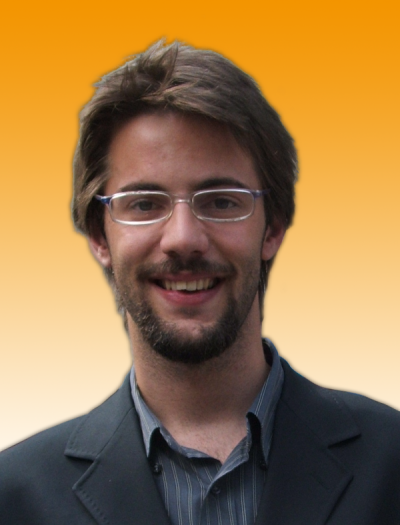
\includegraphics[width=\textwidth]{foto.png}
  \end{minipage}\\[5pt]
  \rule{.8\textwidth}{1pt}
\end{center}
\vspace*{1cm}

\section*{Current Position:}

Project Manager and Software Architect at Si14 SpA

% Iscrizione al Registro Imprese con Partita IVA
% n. 03472460249 con qualifica di ``Consulente nel settore delle % tecnologie dell'informatica''

\section*{Teaching}
\begin{itemize}
\item Master degree in Computer Engineering - 101/110 (Universit\`a degli studi di Padova, 2011);
\item Bachelor degree in Computer Engineering - 92/110 (Universit\`a degli studi di Padova, 2007);
\item Accounting Diploma (I.T.C.G. L. Einaudi di Bassano del Grappa, 2003).
\end{itemize}

\section*{Experiences}
\begin{itemize}
\item CTO at Doochoo Inc;
\item Full-time in the M31 R\&D focused on web services development and new technologies;
\item Thesis care of M31 titled ``SCADA: A monitor and control remote system for industrial devices'';
\item Web application for different customers;
\item Consultant for server design, deploy and maintenance;
\item German Open 2007, ``Humanoids Legue'' with a team from Universit\`a
degli Studi di Padova;
\item Thesis care of Intelligent Autonomous Systems Laboratory titled ``Simultaneous
algorithms of localization and mapping based on Computer Vision'';
\item Written some opensource software, mostly in Ruby and Python.
\end{itemize}

\section*{Computer skills}
\begin{description}
\item[S.O.:] GNU/Linux, Archlinux \& Slackware {\em as first}, advanced knowledge
  in every field, from installation, to configuration, to support-software
  writing. Deep knowledge of {\em bash} scripting.
  Deep knowledge in the server area.
\item[Web:] Deep knowledge of major web frameworks: RubyOnRails (ruby),
  Django (python) and CakePHP (php).
  Ongoing knowledge (with big interest and enthusiasm) on Ember.js framework.
  Excellent experience in everything web-related.
  Deep knowledge of Javascript with excellent experience in jQuery.
  Deep knowledge of major Databases: MySQL, PostgreSQL, MongoDB, Sqlite;
\item[Mobile:] Medium experience in Android Programming (with an app on the store).
\item[Programming:] Excellent knowkedge of Ruby and Python. Deep experience with C++ and QT Framework. Some experience with many other programming
  languages (Java, Perl);
\item[Electronics:] Good knowledge in Atmel microcontroller programming. Basic experience
  in PCB design. Knowledge of Eagle program. Development of a control board for robot
  engines control;
\end{description}

\section*{Working Experience}
\begin{description}
\item[Si14 SpA] February 2013/Now: Project Manager and Software Architect.
    Working on different projects, from high level web frameworks and system management
    to low level programming. I spent 3 months working in Vacaville (CA) in the US
    to provide close support to clients in planning and developing products.
\item[Doochoo Inc] May 2011/February 2013: CTO. Head of developers, assisting
  customers to find the best solutions for customization.
  Delivery of new feature on Pick1.com and deep customizations of the framework
  for clients accounts. Big Data management and analysis. Information extraction and
  custom reports generation.
\item[M31] April 2010/March 2011: Stageaire as software developer at M31. Working with python, ruby and C.
\item[DV Service] January/May 2008: Hardware/Software care.
\item[Zilio SpA] May/October 2007: Research and develompent. Design and
  sell of a linux-based video surveillance system with HD cameras.
\item[Villa Razzolini Loredan] 1999/2004: Week-end waiter.
\item[IALC] June/October 2002: Technical clerk.
\end{description}

% \section*{Active Projects}
% \begin{itemize}
% \item pynokia: program which send sms (and some other interaction)
%   over a bluetooth/cable connection to a Nokia phone. {\em (Python)}\\
% \item videntify: program which gets information from video files. {\em (C)}\\
% %  \url{http://www.ecarlesso.org/works/show/videntify}
% % \item Freesky: scheda controllo motori da servomodellismo,
% %   progettazione, assemblamento e firmware. {\em (Eagle, ARM-C)}\\
% %  \url{http://www.ecarlesso.org/index.php/freesky}
% \end{itemize}

%% \section*{Portfolio WEB}
%% \begin{description}
%% \item[cnssrl.it] Sito dell'azienda CNS srl, con catalogo prodotti
%%   e backend di amministrazione a misura del cliente. Basato su CakePHP
%%   e MooTools\\
%%   \url{http://www.cnssrl.it};
%% \item[ecarlesso.org] Sito personale, in continua crescita. Basato
%%   su CakePhP e MooTools\\
%%   \url{http://www.ecarlesso.org};
%% \end{description}

\section*{Peronal interest}
\begin{itemize}
\item Computer science;
\item Data Structure and Algorithms;
\item Cutting-edge web technologies;
\item {\bf F}ree and {\bf O}pen {\bf S}ource {\bf S}oftware;
\item Math, with special interest in algebra;
\item Interaction between Electronic and Computer Science;
\item October 2009 - Now: Linux User Group of Bassano del Grappa (GrappaLUG).
\end{itemize}

\section*{Language skills}
\begin{description}
\item[Italian:] Mother tongue;
\item[English:] Good level of understanding and writing;
\item[German:] Basic knowledge.
\end{description}


\section*{Me on the Web}
\begin{description}
\item[github.com] most of my opensourced projects and contributions can be found at \url{https://github.com/carlesso/}
\item[LinkedIn] my personal profile on LinkedIn \url{http://www.linkedin.com/in/ecarlesso}
\item[StackOverflow] my stackoverflow profile \url{http://careers.stackoverflow.com/ecarlesso}
\end{description}

\vfill

%% Ai sensi della legge 675/96 (tutela della persona ed altri soggetti
%% rispetto al trattamento dei dati personali), autorizzo al trattamento
%% dei dati personali contenuti nel presente Curriculum Vitae per
%% permettere un adeguata valutazione della mia candidatura finalizzata all'assunzione.
I authorize to deal with information in this document according to the Italian Law n. 675/96

\vspace{1cm}

\footnotesize {This resume is under {\em git}. You can checkout the updated version:}
\begin{verbatim}
    $ git clone git://github.com/carlesso/ecarlesso_cv.git
\end{verbatim}
\end{document}
